\chapter{Omówienie architektury modułu ESP8266}
\label{omowienie_arch}

\section{Opis modułu}
\label{opis_modulu}

Moduł ESP8266 jest tanim modułem umożliwiającym komunikację przez Wi-Fi.
Oferuje on pełną obsługę protokołu TCP/IP a także funkcjonalnościami prostego
32 bitowego mikrokontrolera. Jest naturalnym następcą modułu ESP32. Niska cena 
i mały rozmiar sprawiły że stał się on bardzo popularny wśród konstruktorów 
urządzeń internetu rzeczy.\\

\begin{figure}[H]
	\centering
    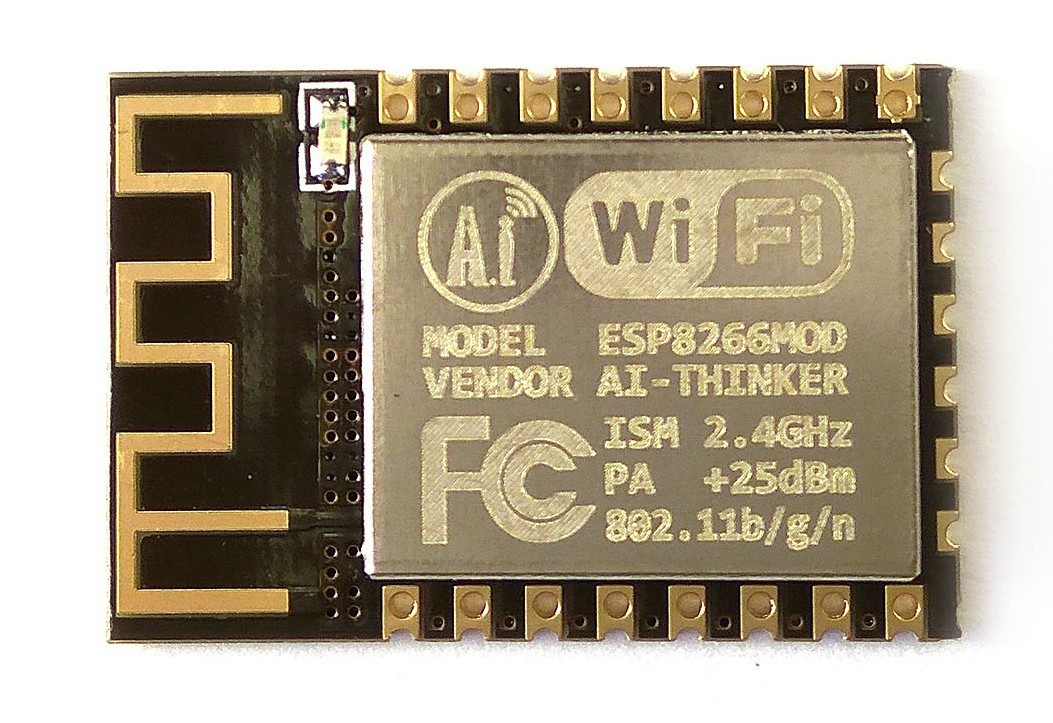
\includegraphics[width=8cm]{./images/esp8266.jpg}
    \caption{Moduł ESP8266 w podstawowej wersji ESP8266-12F firmy AI Thinker}
	\label{screen}
\end{figure}

\subsection{Mikroprocesor}
\label{mikroprocesor}

Na pokładzie modułu ESP8266 znajduje się 32 bitowy mikroprocesor z architektury RISC, 
bazowany na standardzie Xtensa Diamond Standard 106Micro firmy Tensilica.
Jest on domyślnie taktowany zegarem $\num{80}$ MHz, którego częstotliwość można 
zwiększyć do $\num{160}$ MHz. Mikroprocesor został tak skonstruowany aby pobierać 
możliwie jak najmniej energii, przez co dostępne są trzy tryby pracy:
\begin{itemize}
    \item active mode 
    \item sleep mode 
    \item deep sleep mode
\end{itemize}


\subsection{Organizacja pamięci}
\label{pamiec}
Moduł ESP8266 został wyposażony w wbudowaną pamięc SRAM oraz ROM. Rozmiar dostępnej
pamięci RAM dla programu użytkownika w przypadku podłączenia do sieci Wi-Fi w trybie
\textit{station mode} wynosi około $\num{80}$ KiB. Docelowo 
pamięc RAM dostępna dla użytkownika rozpoczyna się od adresu \texttt{3FFE8000h}.
Wewnętrzna pamięć ROM nie jest programowalna a jej rozmiar wynosi $\num{64}$ KiB.
Pamięć ROM mapowana jest w taki sposób że rozpoczyna się od adresu \texttt{40000000h}.

\begin{figure}[H]
	\leftskip3cm
    \includegraphics[width=8cm]{./images/memorymap.pdf}
    \caption{Uproszczona mapa pamięci modułu ESP8266}
	\label{screen}
\end{figure}

Oprócz wbudowanej pamięci, na pokładzie modułu znajduje się również zewnętrzna programowalna
pamięć Flash do przechowywania programów użytkownika. Według dokumentacji, istnieje
możliwość podłączenia pamięci o maksymalnym rozmiarze $\num{16}$ MiB. Zakłada się 
że minimalny rozmiar pamięci Flash powinien wynosić $\num{512}$ KiB w przypadku wyłaczonej
funkcjonalności OTA (Over The Air Update) i $\num{1}$ MiB przy włączonym OTA. Komunikacja
z pamięcią Flash zachodzi przy pomocy interfejsu SPI.

\subsection{Wi-Fi}
\label{wifi}



\subsection{Interfejsy zewnętrzne}
\label{interfejsy}



\section{Organizacja oprogramowania}
\label{organizacja_opr}